\documentclass[a5paper, 10pt, twoside]{book}

\usepackage[utf8]{inputenc}
\usepackage[T1]{fontenc}

\usepackage[francais]{babel}

\usepackage[normalem]{ulem} % texte rayé avec \sout


\usepackage[top=2cm, bottom=2cm, left=2cm, right=2cm]{geometry}

\usepackage{graphicx, wrapfig}
%\DecimalMathComma

% Chevrons Gauche et Droit
\newcommand{\cg}{\guillemotleft~}
\newcommand{\cd}{~\guillemotright}


%%%%%
\title{Les pégus de la ferme\\Tome I\\Panique à la ferme}
\author{Alexis \bsc{Cabodi}\\\\\cg Comment ça on remarque pas du tout\\mes sources d'inspiration ?!\cd}
\date{}
%%%%%
\begin{document}
\maketitle

\renewcommand{\contentsname}{Sommaire}
\tableofcontents

\vfill % Après sur la prochaine page
Des lectures audio seront prochainement disponibles.


\newpage
\newpage

\chapter*{Carte de Péguland}

\newpage
\newpage


\chapter{La disparition (avec des e)}
\cg Ben la poule !\cd

\begin{wrapfigure}{o}{3cm} % Par le plus grand des hasards, elle est à peu près centrée à côté du paragraphe. Sinon spécifier [12]
\begin{center}
Kidnapoule

\includegraphics[width=3cm]{imgs/trobelpoule.png}
\end{center}
\end{wrapfigure}
Tels étaient les derniers mots que Gertrude entendit de Gérard, avant qu'il se fasse enlever par des oies sauvages nourries et vivant à la ferme en échange de bon lait de poule toutes les semaines. Gertrude reconnu bien là Bernard et Wilfried-Constantin, ses deux poules préférées, qui à elles seules arrivaient à soulever Gérard pour l'emmener on ne sait où. Ce qui était sûr, c'est qu'il n'allait pas plus vite qu'un bambin sur un tricycle. Cependant, Gertrude rentra chez elle - dans la grange - et pleura avant de décider d'un plan d'action.

Puis elle décida d'un plan d'action. Le plan se résumait à ceci :
\begin{itemize}
	\item Pleurer à nouveau une dizaine de minutes
	\item Sortir voir si Gérard était encore visible, ce qui semble probable au vu de sa vitesse et de sa corpulence
	\item Prendre le tracteur en panne de Roger le mécanichien
	\item Rouler vers la direction opposée à celle prise par les Bernard et Wilfried-Constantin, afin de se souvenir par où il est parti
\end{itemize}

Après avoir pris le soin d’inonder la grange, elle sortit donc. Sauf qu'elle y est restée 10 minutes et 1 seconde, et ce fut malheureusement trop tard pour apercevoir Gérard.

Elle pleura de nouveau, même si ça ne faisait pas partie de son plan génial.

Une voix lui parvint aux oreilles. C'était Gérard qui disait : \cg Ben... \cd. Ce n'était en fait que l'écho de ce que Gérard a prononcé il y a maintenant un quart d'heure, mais comme elle ne le sut jamais, elle le prit pour un signe de vie venant de son cher frère. Déterminée à le retrouver mort ou vif, elle chaussa ses sandales scandinaves et partit à la recherche du tracteur.

Il est important de préciser à ceux qui n'ont pas regardé la carte que Péguland est une toute petite île du Triangle des Bermudes ignorant totalement l'existence de nos continents. Mais par le plus grand des hasards, certains de nos produits de bonne facture sont perdus lors d'échanges commerciaux hautement sécurisés et sont retrouvés à Péguland. C'est pourquoi un jour, un habitant qu'il est inutile de nommer a jeté une bouteille à la mer contenant la carte présente en début du livre. La curiosité arriva sur les côtes japonaises avant d'être interceptée par un sous-marin russe. Elle devint mondialement connue. Cependant la carte a dû être passée aux rayons gamma car de l'eau s'est infiltrée dans la bouteille pour la simple et bonne raison que l'habitant n'avait pas pensé à mettre de bouchon. Malheureusement cette carte ne fournissait aucune indication utile pour trouver cette île, et jamais nos civilisations ne rencontrèrent la leur.

De retour à la plus célèbre - la seule en fait - ferme de Péguland, on peut voir Gertrude qui fait le tour de la propriété une vingtaine de fois. Aucun tracteur en vue - le comble pour une ferme. Elle décida de retourner pleurer dans la grange. En poussant la grande porte rouge, elle vit enfin le fameux tracteur en panne. Par chance, l'inondation de larmes provoqua un court-circuit qui fit démarrer le tracteur au moment où elle s'assit dessus. Roger qui passait dans le coin fut époustouflé de voir son tracteur redémarrer après 5 années d'immobilité. Aussi décida-t-il de remettre un peu d'essence, qu'il avait siphonnée afin d'éviter les accidents dans la ferme, pour éviter les accidents au milieu de la route. C'est en effet ce qui était arrivé à Roger : il est tombé en panne d'essence alors qu'il passait devant cette modeste ferme - qui couvre 70\% du pays. Ensuite il est tombé en panne tout court, et ne fut jamais capable de faire redémarrer le tracteur. Il prit donc son jerrican en plastique qui avait rouillé et s'approcha du tracteur. Sauf que le tracteur avait aussi disparu. Cette foi l'oie malfaisante s'appelait Gertrude.

Vaillamment, Roger enfourcha un cochon, attacha le jerrican avec un de ses cheveux à la queue du cochon, et partit poursuivre le tracteur en lançant : \cg Allez le cochon lô ! Faudlait rattlapper le tlecteur !\cd, ce sur quoi le cochon couina et fonça en direction du tracteur.

Comme tout le monde le sait, un cochon, aussi grassouillet soit-il, va bien plus vite qu'un tracteur, sauf si ce dernier a des jantes en laiton. Roger étant expert en rodéo de cochon, et le tracteur n'ayant carrément pas (et non \cg plus\cd) de jantes, il rattrapa le tracteur en moins d'un an. Pour préciser les choses, on pourra même dire moins d'un mois. Et pour les plus curieux à l'aise avec les nombres très petits, c'est très exactement en 1/32 768\textsuperscript{ème} de seconde qu'il rattrapa le tracteur et Gertrude. C'est du moins ce qu'indiquait sa montre à quartz de marque \cg Made in China\cd, qu'il a trouvée en train de suffoquer sur une plage de Péguland. C'était une rencontre émouvante et la petite chose avait avalé un sac en plastique, plutôt que de se ranger soigneusement dedans. Depuis ce jour, Roger garda précieusement la montre à sa cheville droite, même s'il s'est avéré que son quartz avait rendu l'âme.

\chapter{À la recherche de Gérard}
\section{Mais où est Gérard ?}
Gérard l'agriculteur est un flemmard de première (classe à laquelle il a arrêté ses études) : voici comment se découpe son emploi du temps\footnote{Oui j'aime les listes inutiles} :
\begin{itemize}
	\item 40\% de son temps à dormir dans son lit, dont 10\% avec Gertrude avant qu'elle aille sur le canapé, ne supportant plus ses ronflements
	\item 3,1415926535\% à s'occuper de la ferme
	\item 30\% en siestes en tout genres
	\item 50\% à manger et/ou à boire
\end{itemize}

Quelle ne fut pas sa joie lorsqu'il se réveilla - après une longue sieste durant le trajet - et découvrit que ses ravisseurs l'avaient abandonné dans un endroit tout bonnement charmant avec toute la nourriture qu'il aimait en abondance. Les Kidnapoules\footnote{Le narrateur se trompe tout du long, ce sont bien des poules, ce qu'ont justement remarqué les 2G\footnote{Les 2G est le surnom du couple formé par Gérard et Gertrude}}\footnote{Même si Gérard reste un grand gamin, il faudrait plutôt parler d'adultnapping\footnote{Ce mot n'existe pas officiellement\footnote{L'auteur s'est renseigné sur le sujet avant d'un informer le narrateur.}} ou de Gérarnapping. Donc plutôt que Kidnapoules, on pourrait dire Gérarnapoules, mais ça sonne très mal.}\footnote{Qui rappelons-le sont des oies sauvages.} ont eu tout leur temps libre en captivité pour observer Gérard en train de manger dans le champ derrière la ferme. Ainsi il avait droit à tout un étalage de chips, saucissons et bières de tous les coins de l'île, avec la mention \cg Qualité Carrouf\cd.

\section{Mais que fait Gérard ?}
Gérard est dans une grotte redécorée pour l'occasion du Sud-Ouest de l'île. À Troce pour être précis. En effet, tout ce gavage intensif avait pour but inavoué de lui faire exploser la panse et de le laisser agoniser dans un monticule de sachets de chips au saucisson parfumées à la bière.

\section[Le début de la quête]{Le début de la quête (Miaouss oui la quéqu---)}
\cg GERTRUDE ! beuglait le cochon sur lequel était debout Roger\\
-- Quoi Polky ?\\
-- GERTRUDE ! beuglait le type qui était debout sur le cochon\\
-- Quoi Loger ?\\
-- Où vas-tu ? demanda Roger avec son bel accent citadin\\
-- Dans l'autle dilection d'où qu'ils ont emmené mon mali pour me souv'nir d'où c'est. expliqua Gertrude\\
-- C'était pas plus simple de les suivre ? remarqua fort justement Roger\\
-- Oh ben j'y avions pô pensé ! dit Gertrude après avoir marqué une pause\cd

Et Gertrude arrêta le tracteur.

Et le cochon continua de foncer dans le tracteur.

Et Roger finit dans les bras de Gertrude, laquelle le laissa tomber dans la fange du pré fraîchement arrosé par des cadavres de bouteilles de bière. Les mêmes que celles que boit Gérard. Cela rendit Gertrude gravement triste. C'est pourquoi elle laissa tomber Roger dans la fange du pré fraîchement arrosé par des cadavres de bouteilles de bière, avant de se retourner dans le silence.

Le lendemain, Roger revint avec Porky voir Gertrude. Elle avait passé toute la nuit à pleurer et avait les yeux injectés de sang. Trois jours après, Roger en comprit la cause et nettoya le champ de toutes les bouteilles. Aussitôt Gertrude repris son sourire habituel - un joli poker-face. Mais quand il lui demanda ce qu'ils allaient faire pour Gérard, elle pleura de nouveau quatre jours, pendant que Roger préparait le matériel de survie afin d'être paré à toute éventualité. Il leur manquait malgré tout un objet indispensable : des serviettes. Roger a su qu'il leur en fallait non pas en lisant le \emph{Guide du voyageur galactique}, ouvrage dont seuls certains britanniques ont entendu parler, mais par pure intuition. Le problème est qu'il a oublié la sienne chez lui à Sion et qu'à la ferme on n'avait même pas l'eau chaude, donc l'idée de se laver n'était jamais venue jusqu'ici (quand Roger l'a compris on a eu droit à 3 tentatives de suicide).

Roger alla donc en acheter dans la ville la plus proche. Il rentra bredouille. Mais puisque nous ne sommes pas matérialistes, on évoquera son enrichissement spirituel : tout d'abord il revient avec l'idée d'essayer de songer à penser à prendre de l'argent, pour payer les serviettes. Ensuite, il a aussi l'infime joie d'avoir salué Gérard, qu'il n'a pas vu depuis plus d'une semaine. Joie dont il fit part à Gertrude à son retour.

Lorsqu'il revint de son second aller-retour, il avait enfin les serviettes. Accessoirement, il a de nouveau vu Gérard.

\cg Très bien ! Nous sommes prêt à aller chercher Gérard ? demanda gaiement Roger\\
-- Hum j'pensions qu'oui ! annonca Gertrude\\
-- D'acc on s'casse alors. répliqua Roger qui commence à intégrer la vulgarité de Gertrude. Allons-y let's go ! C'est parti les amis !\cd

Les ravages de la télévision et des dessins animés tout mignons tout roses éducatifs ou de type My Little Pony...
\vfill
\emph{C'est sur ce début de recherche de Gérard que se clot se chapitre sur la recherche de Gérard, merci de votre lecture et à mardi prochain !}

\chapter{La chevauchée vers l'Ouest}
Lorsque Roger voulu chevaucher depuis la première fois en 5 ans son tracteur adoré, il se fit assommer par un mouton fermement maintenu par Gertrude, qui le laissa ensuite tomber dans la fange. Roger s'écroula non pas dans la fange, mais dans la boue et Gertrude en profita pour escalader le tracteur, ce magnifique tracteur rouge traité contre les puces - un problème souvent ignoré par les fermiers et qui cause des ravages chaque année.

À son réveil, la seule chose environnant Roger était son fidèle destrier Porky IV - le père du Porky de l'autre jour. Roger l'enfourcha et partit dans la direction opposée à celle prise auparavant. Cette fois-ci, il a rattrapé son tracteur au bout d'une bonne heure. En effet, bien que ce cochon-là soit très rapide, il a pris un retard immense d'au moins -2,5 fermes\footnote{= 30km. La ferme est une unité de surface représentant la superficie de la ferme de Gérard, c'est à dire 70\% des 2 000 hectares de l'île principale, soit environ 14 km\textsuperscript{2} Les distances sont converties en fermes en les multipliant par la \emph{constante de le champ de Gérard} notée $ConstanteDeLeChampDeG\acute{e}rard$ et qui vaut -1/12 ferme.m\textsuperscript{-1}. Le résultat obtenu est ainsi en dimension supérieure, puisqu'on l'a alors multiplié par bien plus que l'infini. À l'inverse, il faut multiplier par -12 pour obtenir des mètres à partir de fermes. Notons toutefois que ces conversions n'ont pour eux aucun intérêt puisque les mètres n'existent pas, à part quand ils doivent calculer la surface d'un carré.} à cause de son évanouissement, car étrangement, la boue de Péguland fait s'évanouir quiconque plonge sa tête dedans, alors que la fange est beaucoup plus neutre. C'est pourquoi en l'an 12 AVC\footnote{AVant Gérard, il est faux d'écrire AVG, la barre du G a souvent été prise pour une saleté, à tort. Seul leur G ressemble à celui de notre alphabet.} une grande campagne de nettoyage fut lancée à travers l'île pour la débarrasser de toute sa boue, puis de répandre de la fange à la place. Le seul qui trouva débile l'idée de remettre de la terre mouillée juste après subit énormément de railleries mais conserva la boue jetée dans des flacons. Certains racontent qu'il l'utilise comme opium, d'autres comme somnifère et qu'il passe d'excellentes nuit, et même que certains affirment l'avoir vu neutraliser les gardes de la banque nationnale de Sion et les caméras de sécurité, en laissant un mot signalant le manque de sécurité de leur banque. Aujourd'hui, n'étant plus que le grand rival de Gérard l'agriculteur avec sa petite parcelle au Sud-Ouest, il n'a plus de boue.

En y repensant, Roger s'aperçut que cette boue ne pouvait provenir que de chez cet homme. En y repensant une seconde plus tard, Roger avait déjà oublié sa déduction. Il savait juste qu'il devait retrouver son tracteur alors il se remit en route. Tout du moins il voulu se remettre en route, ce qui n'était pas le cas du cochon, exténué de le regarder s'évanouir. La boue n'était pas à mettre en cause, mais plutôt sa faiblesse intellectuelle. Sa déduction lui a complètement lobotomisé le cerveau alors qu'il était de nouveau si proche de son tracteur. À l'instar d'une crise d'hypothermie, son cerveau eu une activité intense. Or Roger ne supporta pas cette grande différence par rapport à son niveau intellectuel habituel et succomba. La violence du choc l'empêcha de reprendre conscience pendant deux jours durant lesquels Gérard cherchait désespérément sa fourche dans sa grotte. Il fut réveillé par un bruit strident et alternatif, qu'il reconnût aussitôt : c'était le bruit qu'émettait son tracteur lorsqu'il... reculait ! Il sauta aussitôt sur ses pieds et couru vers Gertrude qui lui annonça : \cg Ben ton cochon de malheur coulait comme une vôche décapitée et a tapé ce bôton et depuis j'allive pô à avancer.\cd

Roger se frappa le front de désespoir tellement fort que l'onde de choc produite remit en place le levier de vitesse. Devant un tel exploit, Gertrude laissa conduire Roger. Un plaisir fou envahit son corps, jusqu'à ce qu'il s'aperçoive que le choc a en réalité cassé le levier, laissant ainsi le tracteur au point mort. Le plaisir fut remplacé rapidement par de la tristesse, mêlée à de la colère avec une teinte marquée d'envie suicidaire. Heureusement pour tout le monde, il n'y avait plus de boue dans le coin.

Les deux héros ont dû rentrer à pied à la ferme, car Porky IV n'a pas daigné se montrer. Gertrude cru même l'entendre se moquer d'eux d'un rire sournois, sans parvenir à trouver l'origine de son hallucination auditive.



\cg Bon et cette fois tout est bon ? beugla méchamment Roger le lendemain en scellant son sac au fer rouge.\\
-- J'le pensions ben qu'oui. dit Gertrude après avoir vérifié qu'elle avait pris son smartphone.\\
-- Alors on peut y aller, c'est sûr ? Tout le monde a-t-il bien fait ses besoins ? demanda Roger sur un ton pressé.\\
-- {\tiny Hum pas moi}... marmonna le cochon dans sa moustache.\\
-- Tu feras en route, quand on passera sur la miteuse parcelle d'Henry-Gabriel. Et n'essaye même pas de le faire chez Gérard !\\
-- Roh flûte !\cd

Ces trois joyeux lurons se mirent en route à 23h. Gertrude pleura pour rentrer dormir aux alentours de 23h01.

\chapter{Une étrange rencontre}
Roger ouvrit finalement la porte de la maison de la ferme de Gérard, pensant enfin pouvoir se mettre en route une bonne fois pour toute.

\cg Gné le mais fecteul ben lô ! s'exclama Gertrude qui faillit avaler son chewing-gum.\\
-- Bonjour. J'ai une lettre pour... le facteur regarda attentivement l'enveloppe, avec un air dégoûté. "Ma chélie tlop que j'aime de flangine".\cd

Gertrude arracha l'enveloppe des mains du facteur et commença à lire la lettre. Gertrude dit \cg Loger, j'allive pas bien à lile.\cd, alors Roger prit l'enveloppe et en extirpa la pauvre feuille couverte d'une écriture inconnue qu'il donna à Gertrude, qui n'eut rien d'autre à dire que \cg Han c'est pô l'éclitule de mon flélot.\cd. De toutes façons, Gérard ne savait pas écrire. Elle lit alors la lettre, en contemplant la photo :

\begin{wrapfigure}{o}{5cm}
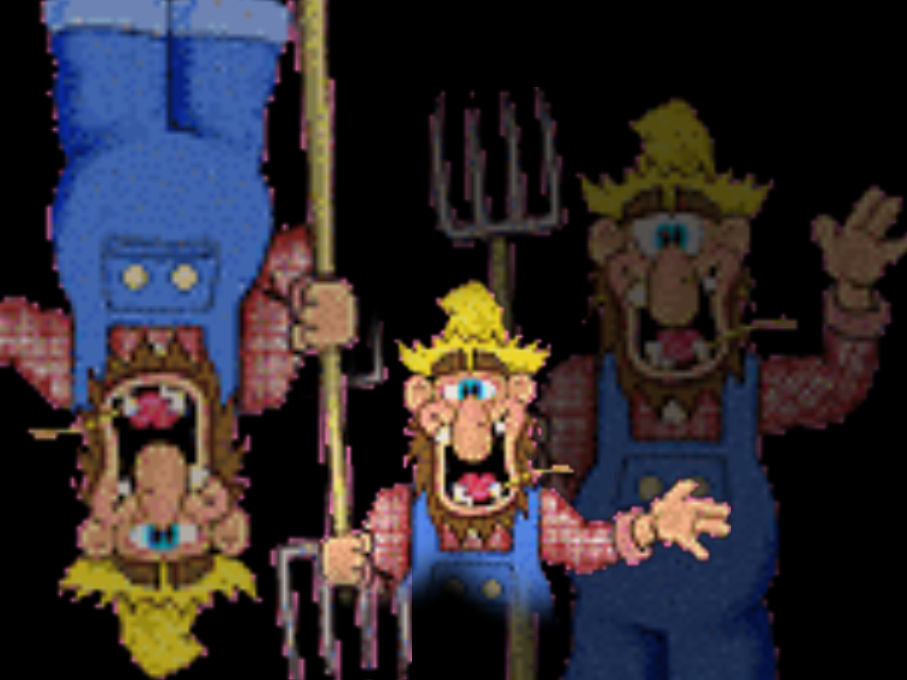
\includegraphics[width=5cm]{imgs/GerardNoir.png}
\end{wrapfigure}
\cg Chel flangine, j'étions tlop content de pouvoil enfin t'éclile. Ben en fait je dicte à \sout{Wiliflied} Wilfried-Constantin mes pensées alols j'espèle que t'allivelas à tout complendle lô. Ici j'ai plutôt la belle vie vu que j'ai toute la bonne lipaille de ma glande glange sans toi poul me gueuler dessus. Donc voilô je voulais te passer le bonjoul, moi j'allions bien ici, même si je suis à Tloce, et que j'ai un mauvais pléssentiment. Mais j'voyons pas c'que nos poules pléfélées poullaient me faile. J'ai vu Loger dans la lue mais je suis quand même lentlé palce que comme j'l'avions dit, c'est bien mieux ici lô. Donc vous plessez pas poul viendle me chelcher hein ?\cd

En face de \cg Signé :\cd il y avait une tache ressemblant orbitalairement\footnote{Orbitalairement, représentant une orbite généralement circulaire synonyme d'obésité, signifie \cg en gros\cd, voire \cg en très le beaucoup gros\cd} à une croix, mais personne n'osait l'affirmer.

Roger se demanda comment les Kidnapoules ont pu écrire ça sans même faire attention aux méfiances que Gérard a à leur égard. Mais cela ne sembla choquer personne d'autre.

\cg Bon ben melci fecteul. J'étions heuleuse d'applendle que mon idiot de mali va biéng. dit Gertrude pour combler le silence qui s'était installé après la lecture.\\
-- Oh mais je ne vais pas me contenter d'un simple \cg melci\cd. Je pourrais repartir avec par exemple... votre tracteur ? dit le facteur avec son regard lubrique posé sur le tracteur.\cd

Roger considéra la proposition. Il pensa que s'il acceptait cette offre, et qu'il se tirait immédiatement, le facteur n'aurait d'autre choix que de faire ce qu'il n'a pas su faire en 5 ans : réparer comme il faut le tracteur. N'osant pas imaginer ce que le facteur voudrait s'il répondait négatif, il a donc accepté et lui a laissé les clés du tracteur, c'est à dire un bout de scotch, pour maintenir deux fils en contact, que le facteur pris avec étonnement et méfiance.

Roger et Gertrude s'enfuirent en courant en direction de Troce sans les affaires qu'ils venaient d'oublier en voulant vite échappant au facteur. N'ayant donc pas d'eau sur eux, ils furent très rapidement épuisés. Aussi Gertrude s'écroula dans de la boue alors que la grange était encore visible d'où ils étaient. Une voix au loin retentit : \cg Mais c'est quoi ce tracteur pourri qui démarre même pas ?!\cd. Ils se remirent à courir de plus belle, sans que l'on %ne ?
sache pourquoi. Gertrude s'étala de tout son long (et son large) à cause bien évidemment de la boue.

\cg Allez Gertrude, c'est pas l'moment ! dit Roger dans sa course effrénée\\
-- Mein blegh rflflflflfl ! gargouilla Gertrude\\
-- Bon je vais te porter alors. Mais pas longtemps hein !\cd

Ce qu'il fit, mais plus longtemps que ce qu'il avait en tête - pas une seule frame d'IRL. Il avait négligé sa fatigue et commençait à ralentir, lorsqu'il entendit un ronronnement familier : encore celui de son tracteur ! \cg Moi, mécanichien surdoué, n'a rien pu faire en 5 ans pour cette pauvre bête et ce... livreur de papier taché fait tout en si peu de temps ?! Quelle honte !\cd\ pensa si fort Roger qu'on l'entendit à des moins dizaines de fermes. Ne pouvant plus continuer son chemin, il décida d'attendre.

Il aurait fallu au facteur un temps phénoménal pour venir jusqu'à Roger, si bien que ce dernier et Gertrude étaient déjà parfaitement requinqués. Et même plus. En effet, Roger a réalisé qu'il avait obtenu une vision d'aigle, qui lui permit d'apercevoir Porky IV qui mangeait de l'herbe à 3 mètres de lui. Fuir ce facteur fou-furieux ou foncer retrouver Gérard l'alcoolique obèse - ce qui pour Gérard était un pléonasme, puisqu'il grossissait à mesure qu'il buvait (et mangeait) ? Ce dilemme fut brusquement détruit par Gertrude qui, n'ayant manifestement pas reprit tous ses esprits, pointait à côté du cochon en criant \cg Pal lô !\cd. Et la chevauchée sauvage à travers les grandes plaines de Gérard reprit. En tendant l'oreille, on entendait le facteur crier des insultes dans l'espoir de les voir faire demi-tour.
\end{document}